\begin{figure}[htbp]
\centering
\begin{subfigure}[b]{0.95\textwidth}
\centering
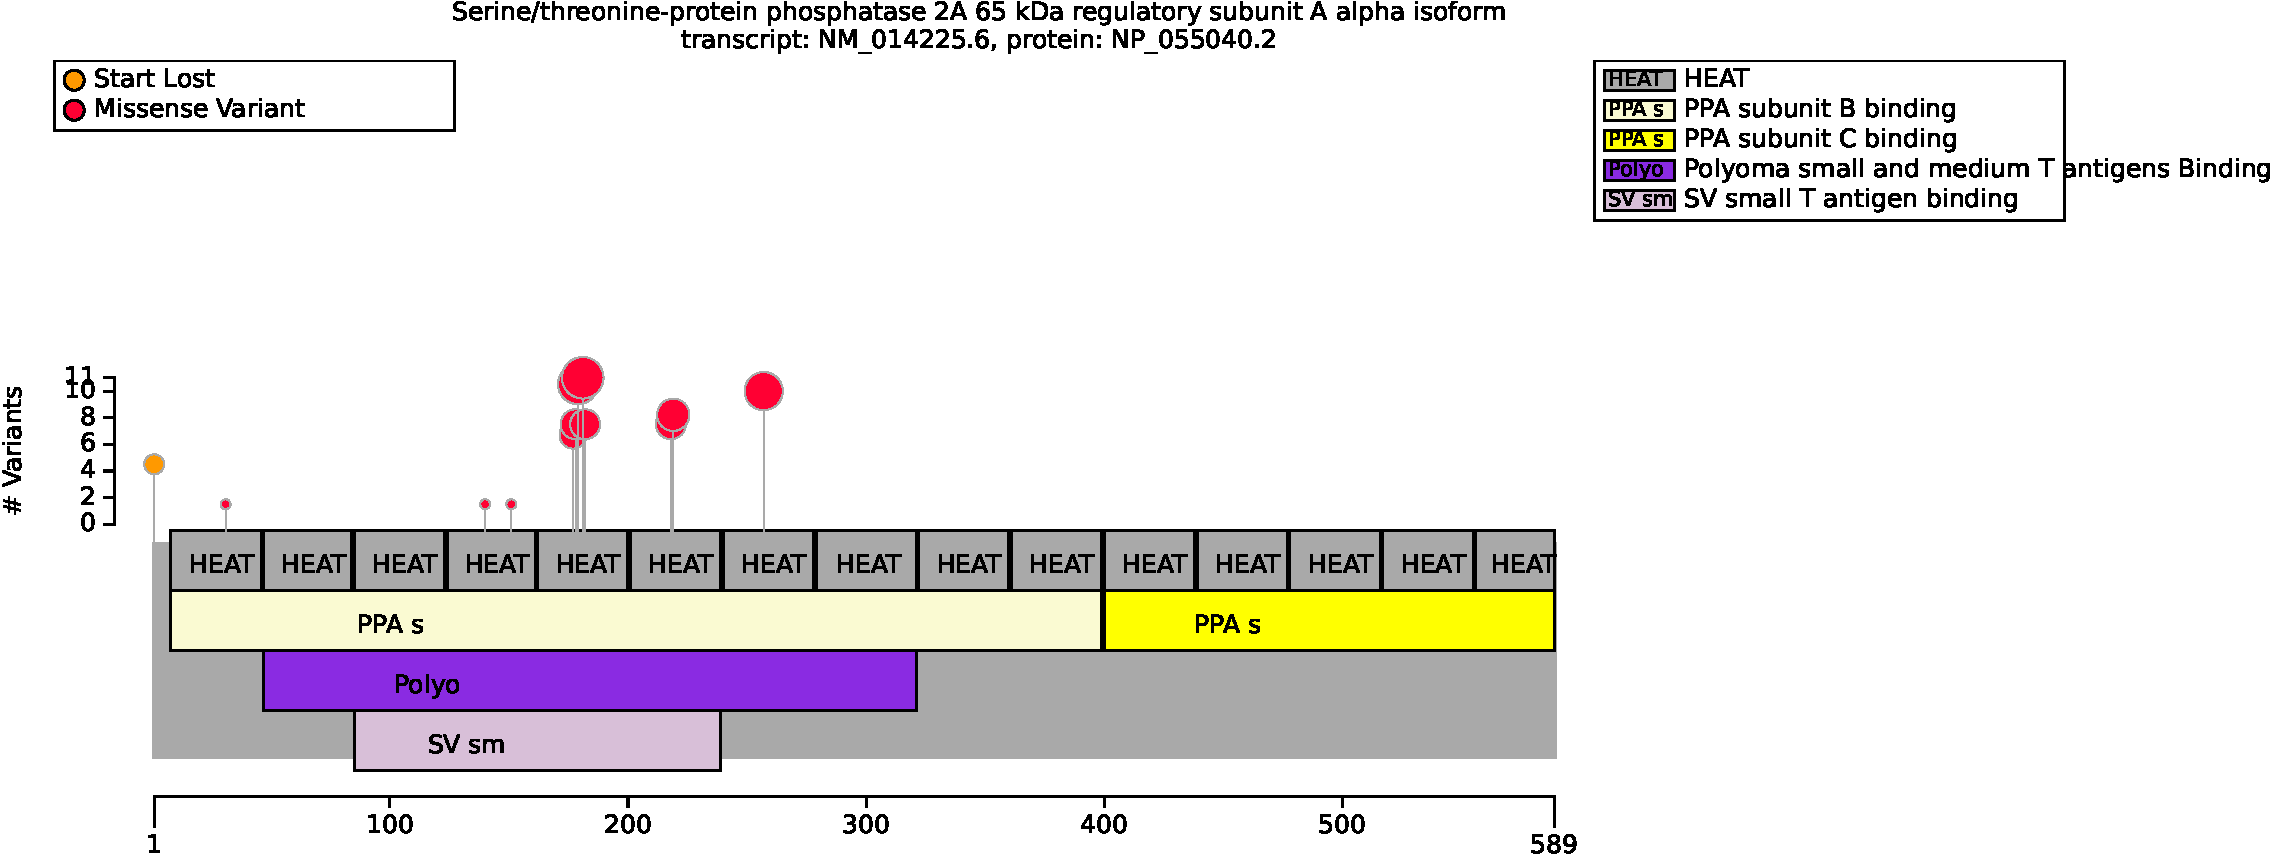
\includegraphics[width=\textwidth]{ img/PPP2R1A_protein_diagram.pdf} 
\captionsetup{justification=raggedright,singlelinecheck=false}
\caption{Distribution of variants in PPP2R1A}
\end{subfigure}

\vspace{2em}

\begin{subfigure}[b]{0.95\textwidth}
\centering
\resizebox{\textwidth}{!}{
\begin{tabular}{llllrr}
\toprule
Genotype (A) & Genotype (B) & total tests performed & significant results\\
\midrule
Absent in COSMIC & Present in COSMIC & 20 & 0\\
Arg182Trp & other & 20 & 0\\
SV40 small T antigen binding & other & 20 & 0\\
\bottomrule
\end{tabular}
}
\captionsetup{justification=raggedright,singlelinecheck=false}
\caption{             Fisher Exact Test performed to compare HPO annotation frequency with respect to genotypes. }
\end{subfigure}

\vspace{2em}

\caption{ The cohort comprised 60 individuals (24 females, 32 males, 4 with unknown sex). A total of 52 HPO terms were used to annotate the cohort. Disease diagnosis: Houge-Janssen syndrome 2 (OMIM:616362). No statistically significant results identified. A total of 60 unique variant alleles were found in \textit{PPP2R1A} (transcript: \texttt{NM\_014225.6}, protein id: \texttt{NP\_055040.2}).}
\end{figure}
